% Python 入门

到 2019 年, 在一些排名中, Python 已经成为最流行的语言, 无论是在科学计算还是在计算机领域都有大量的使用者. 本书中我们主要介绍 python 在科学计算中的应用.

如果不想安装软件可以直接使用用浏览器访问 \href{https://jupyter.org/}{Jupyter Notebook} 运行 Python 程序, 要在本地使用 Python 推荐安装 Anoconda. 以下我们用前者进行讲解. Jupyter Notebook 的优点是交互式编程, 即每输入一个命令都可以立即执行(快捷键 Shift + Enter), 利于学习和实验.

\subsection{作为计算器}
请在 Jupyter Notebook 中尝试输入以下命令并执行(运行结果略). Python 程序使用 \verb|#| 注释一行,  或者用两个 \verb|"""| 注释多行. 注释是为了辅助人阅读代码, 不会被机器执行.

四则运算
\begin{lstlisting}[language=python]
2 + 2
\end{lstlisting}
\begin{lstlisting}[language=python]
123 / 456
\end{lstlisting}
幂运算
\begin{lstlisting}[language=python]
3 ** 2
\end{lstlisting}
整数除法, 即相除再向下取整
\begin{lstlisting}[language=python]
4 // 3
\end{lstlisting}
求余
\begin{lstlisting}[language=python]
4 % 3 # 使得 a == a // b + a % b 恒成立
\end{lstlisting}
使用括号
\begin{lstlisting}[language=python]
(123 - 234*2)**2 / (34 + 54**4)
\end{lstlisting}
各种常见的数学函数都在 math 模块中, 需要加载.
\begin{lstlisting}[language=python]
import math
\end{lstlisting}
使用模块中的函数, 要在前面加上模块名和一点. 例如开方 (square root)
\begin{lstlisting}[language=python]
math.sqrt(284)
\end{lstlisting}
自然指数函数
\begin{lstlisting}[language=python]
math.exp(5.1)
\end{lstlisting}
这样做虽然略显麻烦, 但可以区分不同模块中同名函数. 在确保没有冲突的情况下我们也可以用以下方法加载模块中的指定函数, 如
\begin{lstlisting}[language=python]
from math import sqrt, exp, sin, cos
\end{lstlisting}
现在使用这些函数就不需要 \verb|math.| 的前缀了
\begin{lstlisting}[language=python]
sin(1)
\end{lstlisting}
我们甚至可以用这种方式引入一个模块中所有函数(和其他内容)而无需前缀. 这样做引起名称冲突的可能性更大, 不建议使用.
\begin{lstlisting}[language=python]
from math import *
\end{lstlisting}
从模块中不仅可以引入函数, 还有常数, 例如圆周率和自然对数底(注意 \verb|e| 这种单字母名称很可能会产生冲突, 所以不建议取消 \verb|math.| 前缀)
\begin{lstlisting}[language=python]
sin(pi/2)
\end{lstlisting}
\begin{lstlisting}[language=python]
log(e)
\end{lstlisting}

\verb|math| 模块中的其他常用函数如: 绝对值 (absolute value)
\begin{lstlisting}[language=python]
fabs(-32)
\end{lstlisting}
自然对数
\begin{lstlisting}[language=python]
log(0.5)
\end{lstlisting}
以 10 为底的对数
\begin{lstlisting}[language=python]
log10(1000)
\end{lstlisting}
弧度转为角度
\begin{lstlisting}[language=python]
degrees(pi/2)
\end{lstlisting}

\subsection{变量}
Python 中的\textbf{变量(variable)} 和数学中的不同, Python 的变量可以理解为一个储存数值的容器, 我们可以用等号把一个数值储存在一个变量中. 例如要计算一个长方体的面积, 我们既可以直接把三个数字相乘, 也可以先把这三个数字赋值给三个\textbf{变量}然后相乘
\begin{lstlisting}[language=python]
a = 1
b = 2
c = 3
volumn = a*b*c
\end{lstlisting}
在 Jupyter Notebook 执行这四行发现并没有输出, 无论是一次性执行还是分开执行. 这是因为赋值命令默认不输出结果. 要强制输出结果可以用
\begin{lstlisting}[language=python]
print(volumn)
\end{lstlisting}
或者一次输出多个变量
\begin{lstlisting}[language=python]
print(a, b, c, volumn)
\end{lstlisting}
注意:在python2.x版本中,\verb|print| 是一个关键字,输出内容不需要加括号, python 3.x 中它是一个函数.例如
\begin{lstlisting}[language=python]
print volumn  #2.x
print(volumn) # 3.x
\end{lstlisting}
要强调的是, 这里的等号并不是数学上的等于, 而是\textbf{赋值}, 即把等号右边得到的数值储存在左边的变量中. 在第 4 行执行时, 计算机会先计算等号右边表达式的结果 6, 然后将 6 储存在变量 \verb|volumn| 中. \verb|volumn| 这个变量中并不会包含 \verb|a*b*c| 这个信息, 只储存 6 这个数值. 所以改变 \verb|a, b, c| 后 \verb|volumn| 的值并不会自动改变.

如果要让长方形的某个边长增加 1, 我们可以执行
\begin{lstlisting}[language=python]
a = a + 1
\end{lstlisting}
如果将等号理解为数学上的等于, 这个式子显然是错的. 但正确的理解是, 先把 \verb|a| 当前的值 1 加上 1 得到 2, 然后把 2 \textbf{赋值}给 \verb|a|. 由于我们没有给 \verb|volumn| 重新赋值, 它仍然是 6, 要更新 \verb|volumn|, 只需要重新执行
\begin{lstlisting}[language=python]
volumn = a*b*c
\end{lstlisting}
并用 \verb|print(volumn)| 显示新的值.

等效地, 我们也可以用\textbf{自加运算} \verb|+=|, 将 \verb|a = a + 1| 记为
\begin{lstlisting}[language=python]
a += 1
\end{lstlisting}
注意 \verb|+=| 是一个整体的算符, 中间不能有空格. 类似的运算还有 \verb|-=|, \verb|*=|, \verb|/=| 等.

\subsection{常用数据类型}
\subsubsection{列表(List)}
List (列表) 是 Python 中使用最常用的的数据类型之一.列表中元素的类型可以不相同,它支持数字,字符串甚至可以包含列表.列表是写在方括号 \verb|[]| 之间、用逗号分隔开的元素列表.
\begin{lstlisting}[language=python]
list1 = [1,2,3,4]
list2 = ['a','b',1,3]
print (list1)            # 输出完整列表
print (list1[0])         # 输出列表第一个元素
print (list2[1:3])       # 从第二个开始输出到第三个元素
print (list2[2:])        # 输出从第三个元素开始的所有元素
print (list2 * 2)    # 输出两次列表
\end{lstlisting}
输出为:
\begin{lstlisting}[language=python]
[1, 2, 3, 4]
1
['b', 1]
[1, 3]
['a', 'b', 1, 3, 'a', 'b', 1, 3]
\end{lstlisting}
\subsubsection{元组(Tuple)}
元组(tuple)与列表类似,不同之处在于元组的元素\textbf{不能修改}.元组写在小括号 \verb|()| 里,元素之间用逗号隔开.元组中的元素类型也可以不相同:
\begin{lstlisting}[language=python]
tup1 = (1,2,3,4)
tup2 = ('a','b',1,3)
print(tup1)            # 输出完整元组
print (tup1[0])         # 输出元组第一个元素
print (tup2[1:3])       # 从第二个开始输出到第三个元素
print (tup2[2:])        # 输出从第三个元素开始的所有元素
print (tup2 * 2)
\end{lstlisting}
输出
\begin{lstlisting}[language=python]
(1, 2, 3, 4)
1
('b', 1)
(1, 3)
('a', 'b', 1, 3, 'a', 'b', 1, 3)

\end{lstlisting}
\subsubsection{字典(Dictionary)}
字典是无序的对象集合.字典当中的元素是通过键来存取的,用 \verb|{}| 标识,它是一个无序的 \verb|key:value| 的集合, \verb|key| 和 \verb|value| 分别译成\textbf{键}和\textbf{值}. \verb|key| 必须使用不可变类型. 在同一个字典中, \verb|key| 必须是\textbf{唯一}的.例如统计一个班学生的成绩可以使用字典表示.
\begin{lstlisting}[language=python]
scores = {'语文': 89, '数学': 92, '英语': 93}
print(scores['语文'])
\end{lstlisting}
输出:
\begin{lstlisting}[language=python]
89
\end{lstlisting}
\subsection{函数}
Python 中的函数与数学中的函数不完全一样, 函数可以有若干个输入变量和输出变量(也可以没有). 下面我们定义一个简单的函数来计算长方形的面积
\begin{lstlisting}[language=python]
def f(a, b, c):
    volumn = a*b*c
    return volumn
\end{lstlisting}
这段代码用到了两个 Python 的\textbf{关键字(keyword)} \verb|def| 和 \verb|return|. 关键字是指在程序中有特殊含义的单词, 不能作为变量名和函数名的名称. 其中 \verb|def| 用于定义函数, \verb|f| 是函数名, \verb|a|, \verb|b| 和 \verb|c| 分别是函数的\textbf{输入变量(argument)}. 冒号以后是\textbf{函数体}, 可以有若干行命令. 注意这些命令前面必须有\textbf{缩进(indentation)}.  在以上代码中, 函数体的第一行计算面积, 第二行将用关键字 \verb|return| 将计算的结果作为输出并退出函数.

现在我们可以使用这个函数, 使用方法和 \verb|sin|, \verb|sqrt| 等数学函数一样, 只是不同输入变量要用逗号隔开.
\begin{lstlisting}[language=python]
V = f(1.2, 3.4, 6)
print(V)
\end{lstlisting}

\subsection{数组}
我们这里使用 \verb|numpy| 模块中的数组. \verb|numpy| 是数值计算中一个常用的模块, 主要用于处理各种数组(或矩阵). \verb|numpy| 提供的是ndarray对象,即n维数组对象. 这里介绍另一种 import 的方式
\begin{lstlisting}[language=python]
import numpy as np
\end{lstlisting}
这相当于给 \verb|numpy.| 指定一个更简单的名字 \verb|np.|, 方便了使用. 你也可以把 \verb|np| 替换成其他名字. 上文使用 \verb|math| 模块时也可以使用
\begin{lstlisting}[language=python]
import numpy as m
\end{lstlisting}

要创建一个一维数组(或者叫做行矢量), 如
\begin{lstlisting}[language=python]
a = np.array([1, 2, 3])
\end{lstlisting}
这个数组有三个元素, 每个元素相当于一个独立的变量. 要获取第 \verb|i| 个元素的值, 用 \verb|a[i]|, 如
\begin{lstlisting}[language=python]
a[0]
\end{lstlisting}
注意索引 \verb|i| 从 0 开始而不是 1. 所以第一个元素索引为 0, 第二个索引为 1 等等.

显示整个数组
\begin{lstlisting}[language=python]
print(a)
\end{lstlisting}
要获取数组的一部分
\begin{lstlisting}[language=python]
a[1:2]
\end{lstlisting}
注意:python对数组部分索引获取的时候,不会获取索引范围的最后一个索引值, 即上面这个命令只会得到 \verb|a[1]| 的值为2, 而没有 \verb|a[2]| 的值.

要间隔一个步长获取数组的一部分,可以使用
\begin{lstlisting}[language=python]
a = np.array([1,2,3,4,5,6,7,8])
a[1:6:2]
\end{lstlisting}
括号中的第三个参数表示步长,2表示隔一个元素取一个元素,上述代码取出 \verb|a| 中第 1 个(注意不是第 0 个),第  3 个,第 5 个值, 返回结果为 2,4,6.

创建一个二维数组,如
\begin{lstlisting}[language=python]
b = np.array([[1, 2, 3, 4],[4, 5, 6, 7], [7, 8, 9, 10]])
\end{lstlisting}
数组的大小可以通过其 \verb|shape| 属性获得. 例如获取 \verb|a| 和 \verb|b| 的数组大小,
\begin{lstlisting}[language=python]
a.shape
b.shape
\end{lstlisting}
最终会得到返回值为
\begin{lstlisting}[language=python]
(8,)
(3, 4)
\end{lstlisting}
注意到返回值都有一个小括号,说明返回值类型为一个\textbf{元组类型}. 数组 \verb|a| 的shape只有一个元素,因此它是一维数组.而数组 \verb|c| 的shape有两个元素,因此它是二维数组,其中第0轴的长度为3,第1轴的长度为4.


修改数组的shape属性,在保持数组元素个数不变的情况下,改变数组每个轴的长度.下面的例子将数组 \verb|c| 的shape改为 \verb|(4,3)|,注意从 \verb|(3,4)| 改为 \verb|(4,3)| 并\textbf{不是对数组进行转置\upref{Mat}},而只是改变每个轴的大小,数组元素在内存中的位置并没有改变:
\begin{lstlisting}
b.shape = 4,3
print(b)
\end{lstlisting}
返回
\begin{lstlisting}
array([[ 1, 2, 3],
[ 4, 4, 5],
[ 6, 7, 7],
[ 8, 9, 10]])
\end{lstlisting}
这种操作会永久的改变原数组的shape. 当某个轴的元素为-1时,将根据数组元素的个数自动计算此轴的长度,因此下面的程序将数组 \verb|b| 的shape改为 \verb|(4,3)|:
\begin{lstlisting}[language=python]
c.shape = 4,-1
\end{lstlisting}
另外,通过reshape方法,可以创建一个改变了尺寸的新数组,原数组的shape保持不变.例如
\begin{lstlisting}[language=python]
d = b.reshape((4,3))
print(b)
print(d)
\end{lstlisting}
返回
\begin{lstlisting}[language=python]
array([[1, 2, 3, 4],
[4, 5, 6, 7],
[7, 8, 9, 10]])

array([[ 1, 2, 3],
[ 4, 4, 5],
[ 6, 7, 7],
[ 8, 9, 10]])
\end{lstlisting}
其实数组 \verb|b| 和 \verb|d| 其实共享数据存储内存区域,因此修改其中任意一个数组的元素也会同时修改另外一个数组的内容. 例如,
\begin{lstlisting}[language=python]
b[0]=999
print(b)
print(d)
\end{lstlisting}
输出
\begin{lstlisting}[language=python]
array([[999, 2, 3, 4],
[4, 5, 6, 7],
[7, 8, 9, 10]])

array([[ 999, 2, 3],
[ 4, 4, 5],
[ 6, 7, 7],
[ 8, 9, 10]])
\end{lstlisting}


\subsubsection{一些常用的创建数组的 numpy 函数}
\verb|arange| 函数通过指定开始值、终值和步长来创建一维数组,注意数组\textbf{不包括}终值:
\begin{lstlisting}[language=python]
np.arange(0,10,1)
array([ 0,1, 2, 3, 4, 5, 6, 7, 8, 9])
\end{lstlisting}

\verb|linspace| 函数通过指定开始值、终值和元素个数来创建一维数组,可以通过 \verb|endpoint| 关键字指定是否包括终值,默认是包括终值:
 \begin{lstlisting}[language=python]
np.linspace(0,1,10)
array([0.        , 0.11111111, 0.22222222, 0.33333333, 0.44444444,
       0.55555556, 0.66666667, 0.77777778, 0.88888889, 1.        ])
 \end{lstlisting}

\verb|zeros| 创建全0数组
\begin{lstlisting}[language=python]
np.zeros(3)
array([0., 0., 0.])
np.zeros((3,5))
array([[0., 0., 0., 0., 0.],
       [0., 0., 0., 0., 0.],
       [0., 0., 0., 0., 0.]])
\end{lstlisting} 
另外, \verb|ones|, \verb|eye|创建全1数组,对角元为1的数组,用法与\verb|zeros|类似.


\subsubsection{矩阵的操作}
下面分别介绍对矩阵\upref{Mat}进行一些常见的操作处理,包括转置,拼接,翻转,内积\upref{Dot},外积,计算本征值\upref{MatEig},行列式\upref{Deter},逆矩阵\upref{InvMat},等等在python中的实现.
\begin{lstlisting}[language=python]
A = [1, 2, 3]
B = [[2, 1, 4],[2, 2, 3],[1, 1, 3]]
C = [4, 5, 6]
\end{lstlisting}
转置
\begin{lstlisting}[language=python]
np.transpose(B)
\end{lstlisting}
拼接
\begin{lstlisting}[language=python]
D = np.concatenate((A,C)) # Concatenate vectors
print(D)
[1 2 3 4 5 6]
\end{lstlisting}
左右或者上下翻转矩阵, 字母 \verb|u, d, l, r| 分别是 up, down,  left, 和  right的缩写.
\begin{lstlisting}[language=python]
D = np.flipud(A) 
print(D)
E = np.fliplr(B) 
print(E)
\end{lstlisting}
输出
\begin{lstlisting}[language=python]
[3 2 1]
array([[4, 1, 2],
       [3, 2, 2],
       [3, 1, 1]])
\end{lstlisting}
内积(也叫点乘)\upref{Dot},外积(也叫张量积)
\begin{lstlisting}[language=python]
D = np.dot(A,C) 
print(D)
D = np.outer(A,C) # Outer product
print(D)
\end{lstlisting}
输出
\begin{lstlisting}[language=python]
32
[[ 4  5  6]
 [ 8 10 12]
 [12 15 18]]
\end{lstlisting}
计算本征值\upref{MatEig},逆矩阵\upref{InvMat},行列式\upref{Deter}
\begin{lstlisting}[language=python]
D = np.linalg.eigvals(B) 
print(D)
D = np.linalg.inv(B)
print(D)
D = np.linalg.det(B)
print(D)
\end{lstlisting}
随机数,例如产生0-1之间的随机数
\begin{lstlisting}[language=python]
D = np.random.rand(3,5) 
print(D)
\end{lstlisting}
创建其他随机数方法类似,例如正态分布随机数用 \verb|np.random.randn| 函数.



\subsection{循环语句}
我们经常需要对某个操作重复执行多次,可以用 \verb|for| 循环,例如输出$1$到$3$的平方:
\begin{lstlisting}[language=python]
for i  in range(1,4):
    print(i,i**2)
\end{lstlisting}
输出
\begin{lstlisting}[language=python]
1 1
2 4
3 9
\end{lstlisting}
注意,python中用缩进来表示代码的范围,通常为一个 tab 制表符(即键盘上的 TAB 键), 或者四个空格缩进; \verb|for| 循环后面\textbf{冒号}必不可少. \verb|for| 循环还可以遍历一个列表, 对每个元素执行相同的操作.例如
\begin{lstlisting}[language=python]
A = np.array([3, 2, 4, 5, 1, 76])
for aa in A:
    print(3*aa)
\end{lstlisting}
这里对列表每一个元素扩大3倍. 如果用不得循环指标的时候可以用下划线代替:
\begin{lstlisting}[language=python]
for _ in range(3):
    print('Hello Python')
\end{lstlisting}
此时连续输出   \verb|'Hello Python'|  三次.

有时候我们并不知道循环多少次,此时可以用 \verb|while| 循环. 例如找到最小的 $n$,使得
\begin{equation}
\sum_{i=1}^n i^2<50
\end{equation}
成立.它可以通过 \verb|while| 循环实现. 代码如下
\begin{lstlisting}[language=python]
a = 0
sum0 = 0.0
while sum0 < 50:
    a = a + 1
    sum0 = sum0+a**2
    print(a, sum0)
\end{lstlisting}
输出
\begin{lstlisting}[language=python]
1 1.0
2 5.0
3 14.0
4 30.0
5 55.0
\end{lstlisting}

有时我们在程序中做什么将取决于前面步骤的结果.在这种情况下,您可能会发现 \verb|if| 语句很有帮助.假设我想知道一个二次方程$ax^2+bx+c=0$有多少实根.下面的代码根据$a$、$b$和$c$的值告诉我根的数量.
\begin{lstlisting}[language=python]
a = 5
b = 7
c = -1 
D = b**2 - 4*a*c
if D > 0:
    print("two roots")
if D < 0:
    print("no roots")
if D == 0:
    print("one root")
\end{lstlisting}

通常 \verb|if| 可以嵌套使用;循环语句可以与条件判断语句结合使用.例如,一个简单的打分系统:
\begin{equation}
f=\left\{\begin{array}{lc}\begin{array}{c}A,\\B,\\C,\end{array}&\begin{array}{c}x>90;\\x>80;\\x>60.\end{array}\end{array}\right.\\\\
\end{equation}
\begin{lstlisting}[language=python]
x =99
if x>90:
    print('A')
elif x>80:
    print('B')
else:
    print('C')
\end{lstlisting}


\subsection{python绘图库 matplotlib的使用}

python绘图有很多库, 其中matplotlib库是最受欢迎的绘图库.如果熟悉 Matlab\upref{Matlab} 软件的用户,对matplotlib库就很容易上手,因为matplotlib中很多命令命名与用法与matlab十分类似. 首先在使用之前需要导入模块,并取别名plt.
\begin{lstlisting}[language=python]
import matplotlib.pyplot as plt
\end{lstlisting}
如果使用jupter等在线编辑器,一般需要加入
\begin{lstlisting}[language=python]
% matplotlib inline
\end{lstlisting}
来告诉解释器在浏览器中显示图像.现在我们来看看如何使用这个库.例如在 [0,5] 区间均匀取30个点,分别计算$\sin(x)$与$\exp(x)$,并作图
\begin{lstlisting}[language=python]
A = np.linspace(0,5,30) 
B = np.sin(A)
C = np.exp(-A)
plt.plot(A,B)
plt.hold(True)
plt.plot(A,C)
\end{lstlisting}
上述代码通过 \verb|hold| 把两个图像放在一张画布上面, 如\autoref{Python_fig1} 所示.
\begin{figure}[ht]
\centering
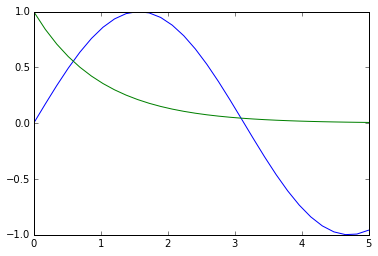
\includegraphics[width=9cm]{./figures/Python_1.png}
\caption{$\sin(x)$与$\exp{x}$} \label{Python_fig1}
\end{figure}


下面给一个综合案例来详细说明这个库的具体使用.结果如\autoref{Python_fig2} 所示.
\begin{lstlisting}[language=python]
import matplotlib.pyplot as plt
import numpy as np
import matplotlib as mpl

mpl.rcParams["font.sans-serif"]=['kaiti']
mpl.rcParams['axes.unicode_minus']=False
plt.subplot(211)
x = np.linspace(0,10,1000)
y = np.cos(x)
x1 = np.linspace(0,10,20)
y1= np.cos(x1)
plt.plot(x,y, ls='-',lw='2',label='曲线图')
plt.scatter(x1,y1,c='b',label='散点图')

plt.xlim(-1,11)
plt.ylim(-1.1,1.1)
plt.xlabel('x轴',fontsize=20)
plt.ylabel('y轴',fontsize=20)
plt.grid(ls='-.',c='r')
#绘制平行坐标轴直线
plt.axhline(y=0,c='g',ls='-',lw=3)
plt.axvline(x=0,c='g',ls='-',lw=3)
#绘制垂直于坐标轴的区域
plt.axvspan(xmin=0,xmax=1,facecolor='y',alpha=0.5)#facecolor或者fcc
plt.axhspan(ymin=0,ymax=0.2,fc='r',alpha=0.5)
#添加箭头注释
plt.annotate('注释内容',
xy=(2,0),
xytext=(3,0.2),
weight='bold',
color='b',
fontsize=20,
arrowprops=dict(arrowstyle='->',
connectionstyle='arc3',
color='b'))
#添加文本注释
plt.text(2,0.8,r'普通文本$\sin(\pi x)$',color='b',weight='bold',fontsize=20)
plt.title('图像标题',fontsize=20)
plt.legend(loc='upper right',title='图例标题',fontsize=20)#里面可有参数
plt.tick_params(labelsize=20)

plt.subplot(212)
plt.plot(x,y,'r-',lw=2)

plt.xticks([0,5,10],[r'$\pi$',r'$2\pi$','C'],rotation=20)
plt.ylim(1,-1)
plt.xlabel('自定义坐标刻度,倒序并旋转',fontsize=20)
plt.text(5,0,'MATPLOTLIB',size=20,rotation=30,
bbox=dict(boxstyle='round',edgecolor='r',facecolor='gray'))
plt.tick_params(labelsize=20)
plt.show()
\end{lstlisting}
先看一下效果图

\begin{figure}[ht]
\centering
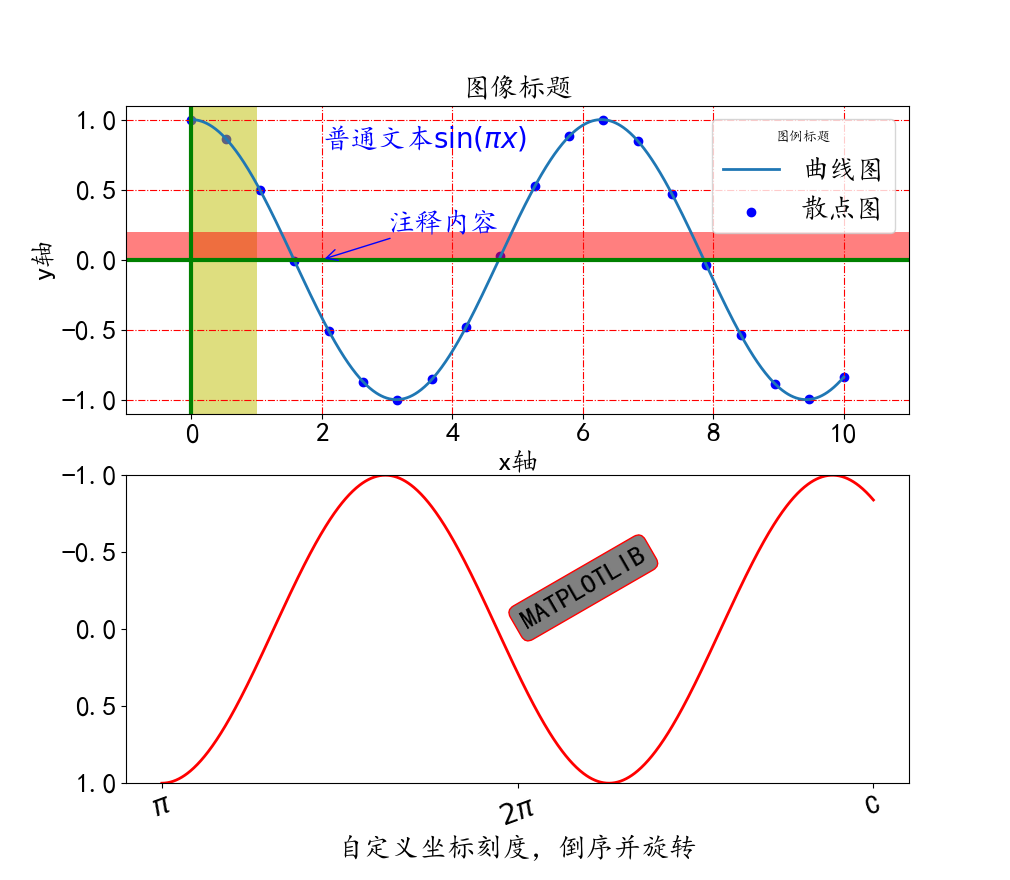
\includegraphics[width=12cm]{./figures/Python_2.png}
\caption{matplotlib库的基本使用} \label{Python_fig2}
\end{figure}

\begin{enumerate}
\item 代码1-3行先导入需要使用的python库
\item 5-6行对字体进行设置,默认情况下中文不显示
\item 7行在一个画布上面划分两行一列的区域,并将后续作图显示在第一个区域
\item 8-11行产生xy数据
\item 12,13行分别绘制曲线图与散点图, \verb|ls| 是 \verb|linestyle| 缩写, \verb|lw|是 \verb|linewidth| 缩写, \verb|c| 是 \verb|color|, \verb|label| 是图例名称
\item 15-19行分别限制坐标轴范围,设置坐标轴名称,已经添加网格线操作.
\item 后续代码,相关说明可以看源码注释部分
\end{enumerate}

